\chapter{Mass fit to \decay{\Bp}{\Dsp\phiz} candidates} 
\label{ch:B2DsPhi}

\minitoc

In this chapter the methodology used to search for \decay{\Bp}{\Dsp\phiz} decays is described.
The branching fraction $\BF(\decay{\Bp}{\Dsp\phiz})$ is constructed by measuring the yield of \decay{\Bp}{\Dsp\phiz} decays relative to the normalisation channel \decay{\Bp}{\Dsp\Dzb}. This ratio is corrected by the ratio of selection efficiencies for the two modes. 
The branching fraction $\BF(\decay{\Bp}{\Dsp\phiz})$ is then determined by multiplying this corrected ratio by externally measured values for the branching fractions $\BF(\decay{\Bp}{\Dsp\Dzb})$ and $\BF(\decay{\Dzb}{\Kp\Km})$, and dividing by $\BF(\decay{\phiz}{\Kp\Km})$. 


{\color{Red}
\begin{itemize}
\item Details of blinding procedure for historic context?
\end{itemize}
}


\section{Fit strategy}
\label{sec:B2DsPhi_fitstrategy}
The strategy used to search for \decay{\Bp}{\Dsp\phiz} is more complicated than the method used to search for \decay{\Bp}{\Dsp\Kp\Km} decays as outlined in Chapter~\ref{ch:B2DsKK}. This is necessary to allow various different signal and background components to be distinguished. In particular, the majority of \decay{\Bp}{\Dsp\Kp\Km} decays now act as a background; those not proceeding via the \phiz resonance must be distinguished from \decay{\Bp}{\Dsp\phiz} decays. 
The ratio of \decay{\Bp}{\Dsp\phiz} and \decay{\Bp}{\Dsp\Dzb} yields is determined using a simultaneous unbinned maximum likelihood fit in a number of different categories. Three sets of categories are used, separating the candidates according to \Dsp meson decay mode, invariant mass of \Kp\Km pair, $m(\Kp\Km)$, and the cosine of an angle $\cos\theta_{K}$. The details and definitions of these categories are listed in Sec~\ref{sec:B2DsPhi_fit_cats}. 
The total extended NLL for this fit is created from the sum of each NLL in each of the categories
\begin{equation}
-\log\mathcal{L}(n_{0}...n_{j},\vec{p}) = \sum_{\alpha} \sum_{\beta} \sum_{\gamma} \left(-\log\mathcal{L^{\alpha,\beta,\gamma}}(n_{0}^{\alpha,\beta,\gamma}...n_{j}^{\alpha,\beta,\gamma},\vec{p}) \right)
\end{equation} 
where $\alpha$, $\beta$ and $\gamma$ represent indexes over the \Dsp mode, $m(\Kp\Km)$ and $\cos\theta_{K}$ categories.
The NLL for each category is defined as before
\begin{equation}
-\log\mathcal{L^{\alpha,\beta,\gamma}}(n_{0}^{\alpha,\beta,\gamma}...n_{j}^{\alpha,\beta,\gamma},\vec{p}) = -\sum_{i}^{N^{\alpha,\beta,\gamma}} \log \left( \sum_{j} n_{j}^{\alpha,\beta,\gamma} f_{j}^{\alpha,\beta,\gamma}(m=m_{i},\vec{p}) \right) + \sum_{j}n_{j}^{\alpha,\beta,\gamma}.
\end{equation} 
As before, $j$ represents the index over each contribution to the fit model, and $i$ represents each of $N^{\alpha,\beta,\gamma}$ entries in the data set for category $\alpha,\beta,\gamma$. 
The composite extended NLL is minimised with respect to the parameters $\vec{p}$ to find the values for which the data is most likely.


\subsection{Simultaneous categories}
\label{sec:B2DsPhi_fit_cats}

The data sample is split into categories primarily to aid the differentiation of different signal and background components that contribute in similar invariant mass ranges.

\subsubsection{\Dsp meson decay mode} 
The three \Dsp decays modes used to reconstruct the signal and normalisation decays (\decay{\Dsp}{\Kp\Km\pip}, \decay{\Dsp}{\pip\pim\pip}, and \decay{\Dsp}{\Kp\pim\pip}) are fitted simultaneously in different categories. This allows the invariant mass distributions for the three modes to vary slightly in ways that could not be easily accounted for if the modes were combined in a single data set. In principle, the widths and resolutions of the \Bp meson mass distributions could vary for the three different modes as a result of the different numbers of pions and kaons in the final state. The background levels also differ between the modes as a result of the smaller branching fractions for \decay{\Dsp}{\pip\pim\pip} and \decay{\Dsp}{\Kp\pim\pip}. This leads to the background from combinations of unrelated tracks having a larger relative contribution.

The \decay{\Dsp}{\Kp\Km\pip} decay mode is additionally split into two further categories; candidates consistent with \decay{\Dsp}{\phiz\pip} decays, and non-\phiz candidates. This exploits the high purity of \decay{\Dsp}{\phiz\pip} decays. 

\subsubsection{Invariant mass of \Kp\Km pair, $m(\Kp\Km)$} 
Three distinct ranges of $m(\Kp\Km)$ invariant mass are used to split the candidates. The first of these corresponds to normalisation \decay{\Bp}{\Dsp\Dzb} candidates within the range $|m(\Kp\Km)-m(\Dzb)|<25 \mevcc$. These are reconstructed separately to the signal decays, unlike in the search for \decay{\Bp}{\Dsp\Kp\Km}, as detailed in Chapter~\ref{ch:selection}. The candidates reconstructed as \decay{\Bp}{\Dsp\phiz} decays are split into two ranges; those within $|m(\Kp\Km)-m(\phiz)|<10\mevcc$, referred to as the \emph{inner \phiz mass category} and those candidates with $10<|m(\Kp\Km)-m(\phiz)|<40\mevcc$, referred to as the \emph{outer \phiz mass category}. These two categories for the signal mode allow contributions from decays that do not proceed via a \phiz meson to be distinguished from those that do. The \emph{inner \phiz mass category} contains 88\% of signal \decay{\Bp}{\Dsp\phiz} candidates, with the other 12\% in the \emph{outer \phiz mass category}. The $m(\Kp\Km)$ invariant mass distribution for simulated \decay{\Bp}{\Dsp\phiz} is shown in Fig~\ref{fig:B2DsPhi_hel_mass_MC}.



%%%%%%%%%%%%%%%%%%%%%%%%%%%%%%%%%%%%%%%%%%%%%%%%%%%%%%%%%%
\begin{figure}[!h]
    \centering
    \begin{subfigure}[t]{0.48\textwidth}
        \centering
        \includegraphics[width=1.0\textwidth]{figs/B2DsPhi/MC_Distributions_mass_B2DsPhi.pdf}
    \end{subfigure}
    \begin{subfigure}[t]{0.48\textwidth}
        \centering
        \includegraphics[width=1.0\textwidth]{figs/B2DsPhi/MC_Distributions_angle_B2DsPhi.pdf}
    \end{subfigure}
    \caption{The distributions of $m(\Kp\Km)$ (left) and $\cos\theta_{K}$ (right) in simulated \decay{\Bp}{\Dsp\phiz} decays. The vertical blue dashed lines represent the boundaries between categories defined in Sec.~\ref{sec:B2DsPhi_fit_cats}. The vertical red lines represent the mass window applied to candidates; those outside the red lines are not included in the data set.}
    \label{fig:B2DsPhi_hel_mass_MC}   
\end{figure}
%%%%%%%%%%%%%%%%%%%%%%%%%%%%%%%%%%%%%%%%%%%%%%%%%%%%%%%%%%


%MC_Distributions_mass_B2DsPhi.pdf



\subsubsection{Helicity angle, $\cos\theta_{K}$} 

The $\decay{\Bp}{\Dsp\phiz}$ decay involves the decay of a pseudoscalar particle to a pseudoscalar and vector particle. Therefore the \phiz vector meson ($J^{P} = 1^{-}$) must be produced longitudinally polarised. For a longitudinally polarised \phiz meson decaying to $\Kp\Km$, the distribution of the angle $\theta_{K}$, defined as the angle that the kaon meson forms with the \Bp momentum in the \phiz rest frame (Fig.~\ref{fig:B2DsPhi_helicity_angle}), is proportional to $\cos^{2}{\theta_{K}}$. The distribution of $\cos{\theta_{K}}$ for $\decay{\Bp}{\Dsp\phiz}$ as determined from simulated events is shown in Fig~\ref{fig:B2DsPhi_hel_mass_MC}. Candidates are split into two categories; $|\cos{\theta_{K}} |> 0.4$ and $|\cos{\theta_{K}} |< 0.4$. These categories contain 93\% and 7\% of the signal respectively.
%%%%%%%%%%%%%%%%%%%%%%%%%%%%%%%%%%%%%%%%%%%%%%%%%%%%%%%%%%
\begin{figure}[!h]
    \centering
    \includegraphics[width=0.48\textwidth]{figs/B2DsPhi/helicityangle.pdf}
    \caption{The angle $\theta_{K}$ (referred to as the helicity angle) is defined to be the angle that the kaon mesons forms with the \Bp meson momentum in the \phiz rest frame.}
    \label{fig:B2DsPhi_helicity_angle}   
\end{figure}
%%%%%%%%%%%%%%%%%%%%%%%%%%%%%%%%%%%%%%%%%%%%%%%%%%%%%%%%%%

This helicity angle is constructed using the momentum of the decay products calculated after the whole decay chain has been refitted with a \Dsp mass and \Bp direction constraint. This significantly increases the fraction of signal events expected in the first of the two categories.


\begin{table}[t]
   \centering
   \begin{tabular}{c|cc}
      \hline
      \multirow{2}{*}{$| m(\Kp\Km) - m_{\phi} |$ (\mevcc)}   & \multicolumn{2}{c}{Helicity Category} \\ 
                       & $|\cos{\theta_{K}} |> 0.4$          & $|\cos{\theta_{K}} |< 0.4$\\ 
      \hline
      $< 10$                           & 82\%           & 6\%                       \\
      (10, 40)                         & 11\%           & 1\%                       \\
      \hline
  \end{tabular}
  \caption{Fractions of $\decay{\Bp}{\Dsp\phiz}$ candidates expected in the helicity and $m(\Kp\Km)$ invariant mass categories of the simultaneous fit. }
  \label{tab:signal_ratios}
\end{table}


\subsection{\decay{\Bp}{\Dsp \Kp \Km} model and assumptions}
\label{sec:B2DsPhi_B2DsKKModel}
The search for \decay{\Bp}{\Dsp\phiz} decays includes a component for \decay{\Bp}{\Dsp\Kp\Km} decays that didn't proceed via a \phiz meson. This is necessary as the search documented in Chapter~\ref{ch:B2DsKK} determined there is a non-zero contribution from these decays in the range of $m(\Kp\Km)$ invariant mass considered here (Fig~\ref{fig:B2DsKK_twobodyprojections}). To avoid overestimating \decay{\Bp}{\Dsp\phiz} signal yield, separate components are included in the fit model for the \decay{\Bp}{\Dsp\phiz} and \decay{\Bp}{\Dsp\Kp\Km} decays. Although the invariant mass distributions of these contributions are identical, they can still be disentangled by exploiting the different fractions of these decays expected in each of the helicity angle and $m(\Kp\Km)$ categories. 
The fractions for the \decay{\Bp}{\Dsp\phiz} signal decays as listed in Table~\ref{tab:signal_ratios} show the decays are concentrated in the \emph{inner \phiz mass category} with $|\cos{\theta_{K}} |> 0.4$. 
To determine similar fractions for \decay{\Bp}{\Dsp\Kp\Km} decays the \laurapp package {\color{Red}(cite)} is used to generate a number of simulation samples for different intermediate resonance models.

Only resonances in the \Kp\Km system are considered as no significant structure is observed in the $m(\Dsp\Km)$ distribution in Fig.~\ref{fig:B2DsKK_twobodyprojections}. As such, all resonances are neutral mesons. The models are generated separately, therefore the effect of interference between any combination of states has been entirely neglected.    
The generated samples are described in the following sections.

\subsubsection{The $\phi(1020)$ resonance} 
Decays proceeding via a $\phiz(1020)$ are produced as a crosscheck. As the simulations generated with \laurapp have not been reconstructed with the full \lhcb detector model, this sample is compared to the existing full simulation samples. The differences in between the fraction of the decays in the different $m(\Kp\Km)$ and $\cos\theta_{K}$ categories in the two samples are taken as a proxy for the potential level of bias introduced by using these generator level samples instead of full simulation. The distribution of these simulated decays in $m(\Kp\Km)$ and $\cos\theta_{K}$ are shown in Fig.~\ref{fig:DsKK_model_phi1020}. This figure also include the Dalitz plot distribution of the decays parametrised with the variables $m^{2}(\Dsp\Km)$ and $m^{2}(\Kp\Km)$.
This resonance is generated with a Relativistic Breit-Wigner line shape~\cite{RelBWPhysRev.49.519}.
%%%%%%%%%%%%%
\begin{figure}[!h]
   \centering   
   \includegraphics[width=0.32\textwidth]{figs/B2DsPhi/phi_phi_mass.pdf}
   \includegraphics[width=0.32\textwidth]{figs/B2DsPhi/phi_Helicity.pdf}
   \includegraphics[width=0.32\textwidth]{figs/B2DsPhi/phi_Dalitz_plot.pdf}
   \caption{The distribution of $m(\Kp\Km)$ (left), Dalitz plot (middle) and the helicity angle $\cos\theta_{K}$ for generated for the $\phiz(1020)$ resonance.} 
   \label{fig:DsKK_model_phi1020}   
\end{figure}
%%%%%%%%%%%%%

\subsubsection{Non-resonant decays}

In addition to \Kp\Km resonances, a non-resonant model is considered. This model is defined to have a uniform amplitude across the allowed phase-space. The distribution in $m(\Kp\Km)$ of \decay{\Bp}{\Dsp\Kp\Km} decays in Fig.~\ref{fig:B2DsKK_twobodyprojections} is not consistent with this model as there are no candidates above $m(\Kp\Km) \sim 1900\mevcc$. However, this component is included in this study for comparative purposes. The distributions of decays generated with this flat model are shown in Fig.~\ref{fig:DsKK_model_NR}. 

%%%%%%%%%%%%%
\begin{figure}[!h]
   \centering   
   \includegraphics[width=0.32\textwidth]{figs/B2DsPhi/NR_phi_mass.pdf}
   \includegraphics[width=0.32\textwidth]{figs/B2DsPhi/NR_Helicity.pdf}
   \includegraphics[width=0.32\textwidth]{figs/B2DsPhi/NR_Dalitz_plot.pdf}
   \caption{The distribution of $m(\Kp\Km)$ (left), Dalitz plot (middle) and the helicity angle $\cos\theta_{K}$ for generated for non-resonant decays.} 
   \label{fig:DsKK_model_NR}   
\end{figure}
%%%%%%%%%%%%%

\subsubsection{The $f_{0}^{0}(980)$ resonance}

The $f_{0}^{0}(980)$ resonance is a light unflavoured $J^{P} = 0^{+}$ state with mass $990\pm20\mevcc$ and width 10--100\mevcc~\cite{PDG2016}. It has been observed to decay to $\Kp\Km$ making it a suitable resonance to consider. Although it's mass is at the lower end of the range considered here, it's significant width allows it to contribute at higher invariant masses. This component is modelled with the Flatt\'{e} line shape~\cite{FLATTE1976224} and the relevant distributions shown in Fig.~\ref{fig:DsKK_model_f0980}.
%%%%%%%%%%%%%
\begin{figure}[!h]
   \centering   
   \includegraphics[width=0.32\textwidth]{figs/B2DsPhi/f0_phi_mass.pdf}
   \includegraphics[width=0.32\textwidth]{figs/B2DsPhi/f0_Helicity.pdf}
   \includegraphics[width=0.32\textwidth]{figs/B2DsPhi/f0_Dalitz_plot.pdf}
   \caption{The distribution of $m(\Kp\Km)$ (left), Dalitz plot (middle) and the helicity angle $\cos\theta_{K}$ for generated for the $f_{0}^{0}(980)$ resonance.} 
   \label{fig:DsKK_model_f0980}   
\end{figure}
%%%%%%%%%%%%%

\subsubsection{The $a_{0}^{0}(980)$ resonance}
The $a_{0}^{0}(980)$ resonance is a light unflavoured $J^{P} = 0^{+}$ state with mass $980\pm20\mevcc$ and width 50--100\mevcc and has been observed to decay to $\PK\Kb$ final states~\cite{PDG2016}. This resonance is also modelled with the Flatt\'{e} line shape and the relevant distributions are shown in Fig~\ref{fig:DsKK_model_a0980}.
%%%%%%%%%%%%%
\begin{figure}[!h]
   \centering   
   \includegraphics[width=0.32\textwidth]{figs/B2DsPhi/a0_phi_mass.pdf}
   \includegraphics[width=0.32\textwidth]{figs/B2DsPhi/a0_Helicity.pdf}
   \includegraphics[width=0.32\textwidth]{figs/B2DsPhi/a0_Dalitz_plot.pdf}
   \caption{The distribution of $m(\Kp\Km)$ (left), Dalitz plot (middle) and the helicity angle $\cos\theta_{K}$ for generated for the $a_{0}^{0}(980)$ resonance.} 
   \label{fig:DsKK_model_a0980}   
\end{figure}
%%%%%%%%%%%%%

\subsubsection{The $f_{0}^{0}(1370)$ resonance}
The $f_{0}^{0}(1370)$ resonance is a light unflavoured $J^{P} = 0^{+}$ state with a mass in the range 1200--1500\mevcc and width in the range 200--500\mevcc. It has been observed to decay to the \kaon\Kb final states. It is modelled with a Relativistic Breit-Wigner line shape and the relevant distributions are shown in Fig.~\ref{fig:DsKK_model_f01370}.
%%%%%%%%%%%%%
\begin{figure}[!h]
   \centering   
   \includegraphics[width=0.32\textwidth]{figs/B2DsPhi/f0_1370_phi_mass.pdf}
   \includegraphics[width=0.32\textwidth]{figs/B2DsPhi/f0_1370_Helicity.pdf}
   \includegraphics[width=0.32\textwidth]{figs/B2DsPhi/f0_1370_Dalitz_plot.pdf}
   \caption{The distribution of $m(\Kp\Km)$ (left), Dalitz plot (middle) and the helicity angle $\cos\theta_{K}$ for generated for the $f_{0}^{0}(1370)$ resonance.} 
   \label{fig:DsKK_model_f01370}   
\end{figure}
%%%%%%%%%%%%%

\subsubsection{The $f_{2}^{0}(1270)$ resonance}
The $f_{2}^{0}(1270)$ resonance is a $J^{P} = 2^{+}$ state with mass $1275.5\pm08\mevcc$ and width $186.7^{+2.2}_{-2.5}\mevcc$ that has been observed to decay to \kaon\Kb final states. This resonance is modelled with a Relativistic Breit-Wigner line shape as shown in Fig.~\ref{fig:DsKK_model_f21270}.

%%%%%%%%%%%%%
\begin{figure}[!h]
   \centering   
   \includegraphics[width=0.32\textwidth]{figs/B2DsPhi/f2_phi_mass.pdf}
   \includegraphics[width=0.32\textwidth]{figs/B2DsPhi/f2_Helicity.pdf}
   \includegraphics[width=0.32\textwidth]{figs/B2DsPhi/f2_Dalitz_plot.pdf}
   \caption{The distribution of $m(\Kp\Km)$ (left), Dalitz plot (middle) and the helicity angle $\cos\theta_{K}$ for generated for the $f_{2}^{0}(1270)$ resonance.} 
   \label{fig:DsKK_model_f21270}   
\end{figure}
%%%%%%%%%%%%%


\subsubsection{The $a_{2}^{0}(1320)$ resonance}
The $a_{2}^{0}(1320)$ resonance is a $J^{P} = 2^{+}$ state with a mass $1318.1\pm0.7\mevcc$ and width $109.8\pm2.4\mevcc$ (both measured in the \kaon\Kb mode) observed decaying to the \kaon\Kb final state. This resonance is modelled with a Relativistic Breit-Wigner line shape and shown in Fig.~\ref{fig:DsKK_model_a21320}.
%%%%%%%%%%%%%
\begin{figure}[!h]
   \centering   
   \includegraphics[width=0.32\textwidth]{figs/B2DsPhi/a2_1320_phi_mass.pdf}
   \includegraphics[width=0.32\textwidth]{figs/B2DsPhi/a2_1320_Helicity.pdf}
   \includegraphics[width=0.32\textwidth]{figs/B2DsPhi/a2_1320_Dalitz_plot.pdf}
   \caption{The distribution of $m(\Kp\Km)$ (left), Dalitz plot (middle) and the helicity angle $\cos\theta_{K}$ for generated for the $a_{2}^{0}(1320)$ resonance.} 
   \label{fig:DsKK_model_a21320}   
\end{figure}
%%%%%%%%%%%%%



\subsubsection{Summary of models}

The fraction of decays expected in each $m(\Kp\Km)$ and $\cos\theta_{K}$ category for the different models considered are tabulated in Table~\ref{table:DsKK_rescfracs}. These are calculated by counting the numbers of entries in the corresponding ranges delineated by the vertical lines in Figs.~\ref{fig:DsKK_model_phi1020}-\ref{fig:DsKK_model_a21320}. For reference the $\phi(1020)$ fractions are included for both the fully simulated decays and those generated with \laurapp. The maximum difference between these fractions is included as a source of systematic uncertainty in Sec.~\ref{sec:B2DsPhi_systuncertainy}.
between For all of the models considered it is clear that the \phiz resonance has significantly different fractions to all of the models considered, allowing the component to be distinguished.   


%%%%%%%%%%%%%%%%%%%%%%%%%%%%%%%%%%%%%%%%%%%%%%%%%%%%%%%%%% 
% Table of things
%%%%%%%%%%%%%%%%%%%%%%%%%%%%%%%%%%%%%%%%%%%%%%%%%%%%%%%%%% 
\begin{table}[!ht]
   \centering
   \begin{tabular}{ c  c  c  c  c }

      \hline
      \multirow{ 2}{*}{\textbf{Model }} & \multicolumn{2}{c}{$|m_{KK}-m_\phi|<10\mev $} & \multicolumn{2}{c}{$10\mev<|m_{KK}-m_\phi|<40\mev$} \\
         & $|\cos{\theta_{K}}|>0.4$ & $|\cos{\theta_{K}}|<0.4$ & $|\cos{\theta_{K}}|>0.4$ & $|\cos{\theta_{K}}|<0.4$ \\
      \hline 
      $\phi(1020)$ \laurapp          & 83.5  &  5.7  & 10.2  &  0.7   \\
      $\phi(1020)$ Full simulation   & 82.4  &  5.9  & 10.9  &  0.8   \\
      \hline
      Non-resonant                   & 16.3  & 11.1  & 45.4  & 27.2   \\
      $f_{0}^{0}(980)$               & 16.5  & 11.2  & 43.3  & 29.0   \\
      $a_{0}^{0}(980)$               & 12.7  &  8.7  & 47.0  & 31.5   \\
      $f_{0}^{0}(1370)$              & 16.1  &  9.6  & 45.0  & 29.3   \\
      $f_{2}^{0}(1270)$              &  8.6  &  6.5  & 59.1  & 25.8   \\
      $a_{2}^{0}(1320)$              &  9.7  &  9.7  & 51.6  & 29.0   \\
      \hline
      Chosen fractions              & 14.6 $\pm$ 1.9  & 10.0 $\pm$ 1.3  & 45.2 $\pm$ 1.9  & 30.3 $\pm$ 1.3   \\
      \hline
   \end{tabular}
   \caption{Fractions of decays expected in each $m(\Kp\Km)$ and $\cos\theta_{K}$ category for the various resonance models considered in Sec.~\ref{sec:B2DsPhi_B2DsKKModel}. }
   \label{table:DsKK_rescfracs}
\end{table}
%%%%%%%%%%%%%%%%%%%%%%%%%%%%%%%%%%%%%%%%%%%%%%%%%%%%%%%%%%

In order to choose suitable fractions for the \decay{\Bp}{\Dsp\Kp\Km} fit component a number of points are considered;

\begin{itemize}
\item Very few events are observed above 2000\mev in the background-subtracted $m(\Kp\Km)$ distribution, therefore the non-resonant model is neglected.
\item No significant peaking structure is observed in the $m(\Kp\Km)$ spectrum so on-shell resonances are neglected
\item The helicity distribution shows no distinctive structure so spin zero states are favoured.  
\item As this is not a full amplitude analysis no attempt is made to include the effects of interference, either between the remaining off-shell resonances or between these and any possible \decay{\Bp}{\Dsp\phiz} decays.
\end{itemize}

These considerations leave the $f_{0}^{0}(980)$ and $a_{0}^{0}(980)$ resonances. The fractions of \decay{\Bp}{\Dsp\Kp\Km} decays that have been used in the fit model are fixed to the average of these two, listed in the final row of Table~\ref{table:DsKK_rescfracs}. Uncertainties are assigned that correspond to half the difference of the two values. These uncertainties are propagated to the $\BF(\decay{\Bp}{\Dsp\phiz})$ branching fraction in Sec.~\ref{sec:B2DsPhi_systuncertainy}. 



\section{Fit components}
\label{sec:B2DsPhi_fitcomponents}

The yields of \decay{\Bp}{\Dsp\phiz} and \decay{\Bp}{\Dsp\Dzb} decays are extracted from the invariant mass distributions of the data sets by representing each component by probability density functions. The components are broadly very similar to those considered in the search for \decay{\Bp}{\Dsp\Kp\Km} decays detailed in Sec.~\ref{sec:B2DsKK_fitcomps}. There are a number of necessary differences:
\begin{itemize}
\item The \Bp invariant mass range considered for both the signal and normalisation channel is expanded to 4900--5900\mevcc. This allows a more stable determination of the various backgrounds contributing in the vicinity of the signal decays. In particular it stabilises the fraction of decays assigned to the combinatorial and partially reconstructed backgrounds at low \Bp invariant mass.   
\item More components are included in the model. This include both the signal mode, \decay{\Bp}{\Dsp\phiz}, and a closely related additional background mode \decay{\Bp}{\Dssp\phiz}. 
\end{itemize}


\subsection{Signal and normalisation decays}
\label{sec:B2DsPhi_signalcomps}

The invariant mass distributions of \decay{\Bp}{\Dsp\phiz} and \decay{\Bp}{\Dsp\Dzb} decays are parametrised using the same DCB function as in the search for \decay{\Bp}{\Dsp\Kp\Km} decays (Sec.~\ref{sec:B2DsKK_sigcomps}):
\begin{equation}
\text{DCB}(m|\mu,\sigma_1,\sigma_2,n,\alpha) = f_\sigma \times \text{CB}(m|\mu,\sigma_1,n,\alpha) + (1-f_\sigma) \times \text{CB}(m|\mu,\sigma_2,n,\alpha),
\label{eq:DoubleBD}
\end{equation}
where the CB function is defined as follows
\begin{equation}
\text{CB}(m|\mu,\sigma,n,\alpha) = \left \{
  \begin{aligned}
    &e^{-\frac{1}{2} \left(\frac{m-\mu}{\sigma}\right)^2} && \text{if}\ \left(\frac{m-\mu}{\sigma}\right) < -|\alpha|\\
    &\frac{\left(\frac{n}{|\alpha|}\right)^n\times e ^{-\frac{1}{2}|\alpha|^2} }{\left(\frac{n}{|\alpha|}-|\alpha| - \frac{m-\mu}{\sigma}\right)^n} && \text{otherwise.}
  \end{aligned} \right.
\end{equation}
Again, $\mu$, $\sigma$, $n$, $\alpha$ and $f_{\sigma}$ are adjustable parameters and $m$ is the \B meson invariant mass observable.
The tail parameter $\alpha$ is fixed to values determined from maximum likelihood fits to simulated candidates for the signal and normalisation decays. The parameter $n$ is fixed to unity in the fits to both simulation and data to increase the stability of the tails.     
The two CB function are allowed have different widths, $\sigma_{1}$ and $\sigma_{2}$, but the ratio $\sigma_{1}/\sigma_{2}$ is fixed from the fits to simulations, as is $f_{\sigma}$ that determines the fractional contribution of the narrower CB function ($\sigma_{1}<\sigma_{2}$). The values determined for each of these fixed parameters are tabulated in Table~\ref{tab:DsPhi_mc_fits}, along with the uncertainty obtained from the fits.

An extra constraint is added to the signal and normalisation DCB functions with respect to the configuration used in the search for \decay{\Bp}{\Dsp\Kp\Km} decays. As the number of signal candidates is likely to be small, the relative width of the narrower signal and normalisation CB functions, $\sigma_{1}(\Dsp\phi) / \sigma_{1}(\Dsp\Dzb)$, is also fixed to values obtained from the fits to simulations.All fixed parameters are determined separately for the different \Dsp decay modes, and the results of the fits to simulated decays are shown in Fig.~\ref{fig:B2DsPhi_signal_fits}.     


%%%%%%%%%%%%%%%%%%%%%%%%%%%%%%%%%%%%%%%%%%%%%%%%%%%%%%%%%% 
\begin{table}[h]
   \centering
   \begin{tabular}{ c c c c }
      \hline
      \multirow{2}{*}{Parameter}                   & \multicolumn{3}{c} {Value} \\
      \cline{2-4}
                                  & \decay{\Dsp}{\Kp\Km\pip}   & \decay{\Dsp}{\Kp\pim\pip} & \decay{\Dsp}{\pip\pim\pip}  \\
      \hline
      %\textbf{$\B \to \Ds \phi$}  &                    &                    &                        \\
      \multicolumn{4}{l} {\decay{\Bp}{\Dsp\phiz}}\\

      \hline
      $\sigma_1/\sigma_2$         & 0.49 $\pm$ 0.01    & 0.47 $\pm$ 0.01    & 0.46 $\pm$ 0.01        \\
      $f_\sigma$                  & 0.80 $\pm$ 0.01    & 0.84 $\pm$ 0.01    & 0.81 $\pm$ 0.01        \\
      $\alpha$                    & 2.76 $\pm$ 0.07    & 3.06 $\pm$ 0.16    & 3.71 $\pm$ 0.23        \\
      $n$                         & 1 $\pm$ 0          & 1  $\pm$ 0         & 1  $\pm$ 0             \\
      \hline
      %\textbf{ }  &                    &                    &                        \\
      \multicolumn{4}{l} {\decay{\Bp}{\Dsp\Dzb}}\\
      \hline
      $\sigma_1/\sigma_2$         & 0.43 $\pm$ 0.01    & 0.42 $\pm$ 0.01    & 0.40 $\pm$ 0.01        \\
      $f_\sigma$                  & 0.88 $\pm$ 0.01    & 0.88 $\pm$ 0.01    & 0.88 $\pm$ 0.01        \\
      $\alpha$                    & 2.91 $\pm$ 0.06    & 3.36 $\pm$ 0.26    & 3.53 $\pm$ 0.25        \\
      $n$                         & 1 $\pm$ 0          & 1 $\pm$ 0          & 1 $\pm$ 0              \\
      \hline 
      $\sigma_{1}(\Dsp\phi) / \sigma_{1}(\Dsp\Dzb)$ & 1.27 $\pm$ 0.02 & 1.31 $\pm$ 0.02 & 1.26 $\pm$ 0.02 \\
      \hline
   \end{tabular}
   \caption{Fixed values obtained in fits to MC used in the model for the signal pdf.} 
   \label{tab:DsPhi_mc_fits}  
\end{table}
%%%%%%%%%%%%%%%%%%%%%%%%%%%%%%%%%%%%%%%%%%%%%%%%%%%%%%%%%% 


%%%%%%%%%%%%%%%%%%%%%%%%%%%%%%%%%%%%%%%%%%%%%%%%%%%%%%%%%%
\begin{figure}[!h]
   \centering
   \begin{subfigure}[t]{1.0\textwidth}
      \centering
      \includegraphics[width=0.40\textwidth]{figs/B2DsPhi/Plot_Signal_Fit_All_B2PhiDs_Ds2KKPi.pdf}
      \includegraphics[width=0.40\textwidth]{figs/B2DsPhi/Plot_Signal_Fit_All_B2D0Ds_Ds2KKPi.pdf}
   \caption{\decay{\Dsp}{\Kp\Km\pip}}
   \end{subfigure}\\
   \begin{subfigure}[t]{1.0\textwidth}
      \centering
      \includegraphics[width=0.40\textwidth]{figs/B2DsPhi/Plot_Signal_Fit_All_B2PhiDs_Ds2PiPiPi.pdf}
      \includegraphics[width=0.40\textwidth]{figs/B2DsPhi/Plot_Signal_Fit_All_B2D0Ds_Ds2PiPiPi.pdf}
      \caption{\decay{\Dsp}{\pip\pim\pip}}
   \end{subfigure}\\
   \begin{subfigure}[t]{1.0\textwidth}
      \centering
      \includegraphics[width=0.40\textwidth]{figs/B2DsPhi/Plot_Signal_Fit_All_B2PhiDs_Ds2KPiPi.pdf}
      \includegraphics[width=0.40\textwidth]{figs/B2DsPhi/Plot_Signal_Fit_All_B2D0Ds_Ds2KPiPi.pdf}
      \caption{\decay{\Dsp}{\Kp\pim\pip}}
   \end{subfigure}\\
   \caption{Invariant mass fits to simulated signal (left) and normalisation (right) decays. The results of maximum likelihood fits using the signal PDFs are over laid, with the total function in black and the two contributing CB shapes in red and blue.}
   \label{fig:B2DsPhi_signal_fits}   
\end{figure}
%%%%%%%%%%%%%%%%%%%%%%%%%%%%%%%%%%%%%%%%%%%%%%%%%%%%%%%%%%


\subsection{Partially reconstructed backgrounds}
\label{sec:B2DsPhi_partrecocomps}

The accurate parametrisation of partially reconstructed backgrounds is particularly important in the search for \decay{\Bp}{\Dsp\phiz} decays as many different processes contribute to the low invariant mass range of the $m(\Dsp\phiz)$ spectrum. These processes involve decays of \Bs, \Bz or \Bp mesons in which the five final state tracks reconstructed in the search for \decay{\Bp}{\Dsp\phiz} decays are only a subset of the background modes final state. 
Typically, processes in which a low momentum pion or photon has not been reconstructed are found closest in mass to the signal decays. Decays of \Bs mesons are particularly dominant as the \Bs meson has a larger mass than the \Bp meson.   


\subsubsection{Backgrounds to the normalisation channel}

The modes \decay{\Bp}{\Dsp\Dstarzb} and \decay{\Bp}{\Dssp\Dzb} can both contribute as partially reconstructed backgrounds to the \decay{\Bp}{\Dsp\Dzb} normalisation mode. These are parametrised using the same PDFs as in the search for \decay{\Bp}{\Ds\Kp\Km} decays, detailed in Sec.~\ref{sec:B2DsKK_norm_partreco}. 

The invariant mass fit range is wider than in the fit to \decay{\Bp}{\Dsp\Kp\Km} candidates, therefore an extra contribution is included in the fit model to account for partially reconstructed \decay{\Bp}{\Dssp\Dstarzb} decays at lower invariant masses.

\begin{description}
\item \textbf{\decay{\Bp}{(\decay{\Dssp}{\Dsp[\piz]})\Dzb} and \decay{\Bp}{\Dsp(\decay{\Dstarzb}{\Dzb[\piz]})}:} these components are modelled by a parabola convolved with a resolution Gaussian. The parabola has a minimum in the centre and doesn't extend beyond endpoints $a$ and $b$
\begin{equation}
f(m|a,b,\sigma,\xi, \delta) = \int_{a}^{b}\left(\mu-\frac{a+b}{2}\right)^{2} \left( \frac{1-\xi}{b-a}\mu + \frac{b\xi-a}{b-a} \right) e^{-\frac{-(\mu-(m-\delta))^{2}}{2\sigma^{2}}} d\mu.
\label{eq:DsPhi_RooHorns}
\end{equation}
These components are shown by the black lines in Fig.~\ref{fig:B2DsPhi_DsD0_partreco}.

\item \textbf{\decay{\Bp}{(\decay{\Dssp}{\Dsp[\Pgamma]})\Dzb} and \decay{\Bp}{\Dsp(\decay{\Dstarzb}{\Dzb[\Pgamma]})}:} these components are modelled by a parabola convolved with a resolution Gaussian. The parabola has a maximum in the centre and doesn't extend beyond endpoints $a$ and $b$
\begin{equation}
f(m|a,b,\sigma,\xi, \delta) = \int_{a}^{b} -(\mu-a)(\mu-b)\left( \frac{1-\xi}{b-a}\mu + \frac{b\xi-a}{b-a} \right) e^{-\frac{-(\mu-(m-\delta))^{2}}{2\sigma^{2}}} d\mu.
\label{eq:DsPhi_RooHills}
\end{equation}
These components are shown by the blue lines in Fig.~\ref{fig:B2DsPhi_DsD0_partreco}.
\end{description}

%%%%%%%%%%%%%%%%%%%%%%%%%%%%%%%%%%%%%%%%%%%%%%%%%%%%%%%%%%
\begin{figure}[!h]
    \centering
    \includegraphics[width=0.80\textwidth]{figs/B2DsPhi/DsD0_part_reco_Shapes.pdf}
    \caption{Partially reconstructed $\Dsp\Dzb$ shapes.}
    \label{fig:B2DsPhi_DsD0_partreco}   
\end{figure}
%%%%%%%%%%%%%%%%%%%%%%%%%%%%%%%%%%%%%%%%%%%%%%%%%%%%%%%%%%


\begin{description}

\item \textbf{\decay{\Bp}{\Dssp\Dstarzb}:} the lower invariant mass range used in this search necessitates including a PDF for \decay{\Bp}{\Dssp\Dstarzb} decays in which two soft particles have been missed, one from each of the excited \D meson decays. It is possible for either a \piz or \Pgamma to be not reconstructed in the decays of both excited \D mesons. Additionally, as this process involves a psecudo-scalar meson decaying to two vector mesons, there should be two distinguishable helicity combinations for each process. This leads to a total of eight PDFs necessary to fully parametrise this contribution. Instead, however, this component is parametrised using a single function of the form given in Eq.~\ref{eq:DsPhi_RooHills}. The endpoints $a$ and $b$ are estimated by combining the effects of missing two neutral particles. The resulting distribution is shown in Fig.~\ref{fig:B2DsPhi_DsstarDstar0_partreco}.
The choice of PDF for this component is found to have negligible effect on the determination of the $\BF(\decay{\Bp}{\Dsp\phiz})$ branching fraction as detailed in Sec~\ref{sec:B2DsPhi_systuncertainy}.

\end{description}

%%%%%%%%%%%%%%%%%%%%%%%%%%%%%%%%%%%%%%%%%%%%%%%%%%%%%%%%%%
\begin{figure}[!h]
    \centering
    \includegraphics[width=0.80\textwidth]{figs/B2DsPhi/DsstarDstar0_part_reco_Shapes.pdf}
    \caption{Partially reconstructed $\Dsp\Dzb$ shapes.}
    \label{fig:B2DsPhi_DsstarDstar0_partreco}   
\end{figure}
%%%%%%%%%%%%%%%%%%%%%%%%%%%%%%%%%%%%%%%%%%%%%%%%%%%%%%%%%%



\subsubsection{Backgrounds to the signal channel}

%The signal channel invariant mass distribution receives contributions from the partially reconstructed modes considered in the search for \decay{\Bp}{\Dsp\Kp\Km} decays. The PDFs determined are 



\begin{description}
\item \textbf{\decay{\Bp}{(\decay{\Dssp}{\Dsp[\Pgamma]})\phiz} and \decay{\Bp}{(\decay{\Dssp}{\Dsp[\piz]})\phiz}:} the decays of \Bp mesons to an excited \Dsp meson and a \phiz meson could contribute to the $m(\Dsp\phiz)$ spectrum at low invariant masses when either a \piz or \Pgamma is missed from the excited meson decay. The resulting invariant mass distribution depends on the mass and spin of the non-reconstructed particle, as well as the helicity state of the \Dssp meson. This background involves the decay of a pseudo-scalar meson to two vector mesons, hence, as a result of angular momentum conservation, there are three helicity states of the \Dssp meson to consider. These are labelled \emph{001}, \emph{010} and \emph{100}. The two transversely polarised states, 100 and 001, have identical invariant mass distributions and are therefore referred collectively as \emph{101}. This leads to a total of four contributions to consider for \decay{\Bp}{\Dssp\phiz} decays. These can be parametrised by parabolas convolved with resolution Gaussians in a similar way to the partially reconstructed backgrounds to the normalisation channel.
These each share the same functional form
\begin{equation}
f(m|a,b,\sigma,\xi, \delta) = \int_{a}^{b} g(\mu,a,b) \left( \frac{1-\xi}{b-a}\mu + \frac{b\xi-a}{b-a} \right) e^{-\frac{-(\mu-(m-\delta))^{2}}{2\sigma^{2}}} d\mu.
\label{eq:DsPhi_DsstarPhi_shapes}
\end{equation}
where $g(\mu,a,b)$ represents the parabola for each of the four components, listed in Table~\ref{tab:DsPhi_DsstarPhi_parabolas}. The resulting invariant mass distributions are shown in Fig.\ref{eq:DsPhi_DsstarPhi_shapes}.

This decay is unobserved, therefore the relative contribution to this decay in nature from the \emph{101} and \emph{010} helicty states is not known. The total PDF for this contribution is made by weighting the \piz and \Pgamma contributions by their corresponding branching fractions, and by assuming that the \emph{101} and \emph{010} helicty states contribute with equally magnitudes. This assumption is varied and included as a source of systematic uncertainty in the $\BF(\decay{\Bp}{\Dsp\phiz})$ determination.
\end{description}
 
%%%%%%%%%%%%%%%%%%%%%%%%%%%%%%%%%%%%%%%%%%%%%%%%%%%%%%%%%% 
\begin{table}[h]
   \centering
   \begin{tabular}{ c c c c c }
      \hline
      Missed particle   & Helicity  & $g(\mu,a,b)$                                      & $a$ (\mevcc) & $b$ (\mevcc)  \\
      \hline
      \piz              & 010       & $\left(\mu - \frac{a+b}{2}\right)^{2}$            & 5026.8       & 5124.8         \\
      \piz              & 101       & $-(\mu - a)(\mu-b)$                               & 5026.8       & 5124.8         \\
      \Pgamma           & 010       & $-(\mu - a)(\mu-b)$                               & 4936.4       & 5220.6         \\
      \Pgamma           & 101       & $(\mu - \frac{a+b}{2})^{2} +(\frac{a+b}{2})^{2} $ & 4936.4       & 5220.6         \\
      \hline
   \end{tabular}
   \caption{Parabolas.} 
   \label{tab:DsPhi_DsstarPhi_parabolas}  
\end{table}
%%%%%%%%%%%%%%%%%%%%%%%%%%%%%%%%%%%%%%%%%%%%%%%%%%%%%%%%%% 


%%%%%%%%%%%%%%%%%%%%%%%%%%%%%%%%%%%%%%%%%%%%%%%%%%%%%%%%%%
\begin{figure}[!h]
    \centering
    \includegraphics[width=0.80\textwidth]{figs/B2DsPhi/DsPhi_part_reco_Shapes.pdf}
    \caption{Partially reconstructed $\Dsp\phiz$ shapes.}
    \label{fig:B2DsPhi_DsPhi_partreco}   
\end{figure}
%%%%%%%%%%%%%%%%%%%%%%%%%%%%%%%%%%%%%%%%%%%%%%%%%%%%%%%%%%


{\color{Blue}
Additionally, the distribution of each shape in the helicity angle described in Section~\ref{subsec:Hel} is approximated to be $\cos^2(\theta)$ for the longitudinally polarized shapes (010) and $\sin^2(\theta)$ for the transversely (101). The fraction in each bin for 010 or 101 is taken from the appropriate integrals of these assumed distributions. 
}

\begin{description}
\item \textbf{\decay{\Bsb}{\Dsp\Km\Kstarz}:} this decay can form a background to \decay{\Bp}{\Dsp\phiz} decays when the soft pion from the \decay{\Kstarz}{\Kp\pim} decay is not reconstructed. The lower bound of the fit range is wide enough that a significant fraction of these decays are retained in the fitted data set. A PDF for this component is determined by reconstructing simulated \decay{\Bsb}{\Dsp\Km\Kstarz} decays through the identical reconstruction and selection steps as the signal. The \roofit class \texttt{RooKeysPDF} is used to create a kernel estimation of the partially reconstructed \Bp mass distribution for the candidates passing the selection. This is shown in Fig.~\ref{fig:B2DsPhi_part_reco_shapes}.

\item \textbf{\decay{\Bsb}{\Dssp\Km\Kstarz}:}
\item \textbf{\decay{\Bsb}{\Dsp\Dsm}:} 
\item \textbf{\decay{\Bzb}{\Dsp\Dm}:} 
\item \textbf{\decay{\Bsb}{\Dssp\Dsm}:} 
\end{description}




%%%%%%%%%%%%%%%%%%%%%%%%%%%%%%%%%%%%%%%%%%%%%%%%%%%%%%%%%%
\begin{figure}[!h]
    \centering
    \begin{subfigure}[t]{0.49\textwidth}
        \includegraphics[width=1.0\textwidth]{figs/B2DsPhi/Bs2Dsa1_4600_5900_Shape.pdf}
        \caption{\decay{\Bsb}{\Dsp} }
    \end{subfigure}
    \begin{subfigure}[t]{0.49\textwidth}
        \includegraphics[width=1.0\textwidth]{figs/B2DsPhi/Bs2DsstKKst_4600_5900_Shape.pdf}
        \caption{\decay{\Bsb}{\Dsp\Kstar\Kp} }
    \end{subfigure}
    \begin{subfigure}[t]{0.49\textwidth}
        \includegraphics[width=1.0\textwidth]{figs/B2DsPhi/Bs2DsDs_4600_5900_Shape.pdf}
        \caption{\decay{\Bsb}{\Dsp\Dsm} }
    \end{subfigure}
    \begin{subfigure}[t]{0.49\textwidth}
        \includegraphics[width=1.0\textwidth]{figs/B2DsPhi/Bs2DsstDs_4600_5900_Shape.pdf}
        \caption{\decay{\Bsb}{\Dssp\Dsm} }
    \end{subfigure}
    \caption{Partially reconstructed mass shapes}
    \label{fig:B2DsPhi_part_reco_shapes}   
\end{figure}
%%%%%%%%%%%%%%%%%%%%%%%%%%%%%%%%%%%%%%%%%%%%%%%%%%%%%%%%%%


\subsection{Combinatorial  backgrounds}
\label{sec:B2DsPhi_combcomps}

Combinations of unrelated tracks form a background to the signal decays and extend across the entire fitted \Bp meson mass range. 
This component is parametrised with an decaying exponential function 
\begin{equation}
f(m|c) = e^{-m\times c},
\end{equation}
where the parameter $c$ controls the slope and $m$ is the observable \Bp meson invariant mass. 
The combinatorial background is the dominant background below the signal events 


\section{Free and constrained parameters}

\section{Fit validation}
\label{sec:B2DsPhi_fitstrategy}

{\color{Red}
\begin{itemize}
\item Toy distributions
\end{itemize}
}

\section{Normalisation and signal fits}




%%%%%%%%%%%%%%%%%%%%%%%%%%%%%%%%%%%%%%%%%%%%%%%%%%%%%%%%%%
\begin{figure}[!h]
    \centering
    \begin{subfigure}[t]{1.0\textwidth}
        \includegraphics[width=1.0\textwidth]{figs/Appendix_FitCategories/canvas_DsD0_merged_both_summed_splitHel_splitKKPi_s21_s21r1_s24_s26.pdf}
    \end{subfigure}
    \caption{Invariant mass fits to \decay{\Bp}{\Dsp\Dzb} candidates}
\end{figure}
%%%%%%%%%%%%%%%%%%%%%%%%%%%%%%%%%%%%%%%%%%%%%%%%%%%%%%%%%%


%%%%%%%%%%%%%%%%%%%%%%%%%%%%%%%%%%%%%%%%%%%%%%%%%%%%%%%%%%
\begin{figure}[!h]
    \centering
    \begin{subfigure}[t]{1.0\textwidth}
        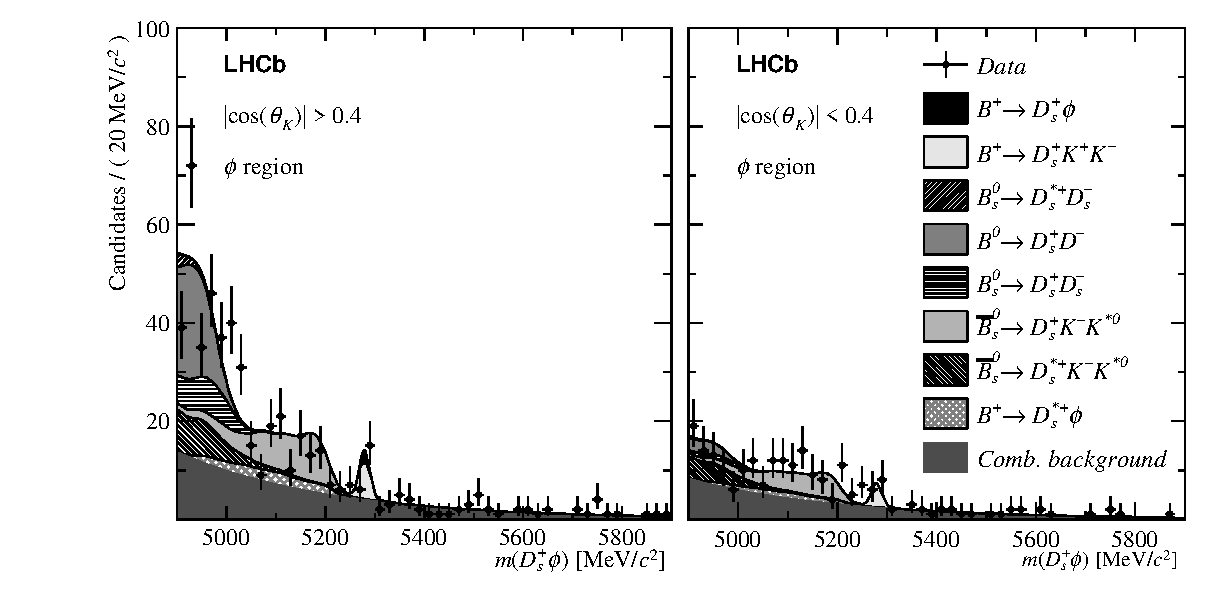
\includegraphics[width=1.0\textwidth]{figs/B2DsPhi/Fig4a.eps}
    \end{subfigure}
    \begin{subfigure}[t]{1.0\textwidth}
        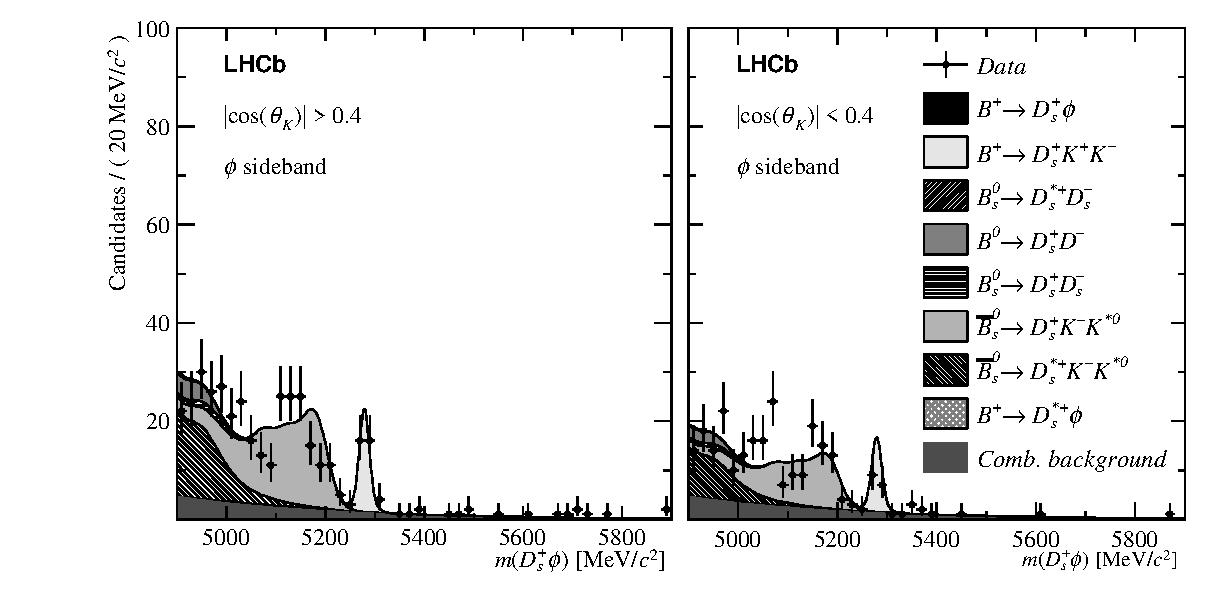
\includegraphics[width=1.0\textwidth]{figs/B2DsPhi/Fig4b.eps}
    \end{subfigure}
    \caption{Invariant mass fits to \decay{\Bp}{\Dsp\phiz} candidates}
\end{figure}
%%%%%%%%%%%%%%%%%%%%%%%%%%%%%%%%%%%%%%%%%%%%%%%%%%%%%%%%%%



\section{Efficiency corrections}
\label{sec:B2DsPhi_effcorrections}


\begin{itemize}
\item Generator Level Efficiencies
\item Trigger Efficiencies
\item Mass Window
\item Cross-feed vetos
\item IP chi2 cuts
\item Charmless Cut
\item MVA Efficiencies
\item PID Efficiencies
\item Total Efficiency
\end{itemize}

{\color{Red}
\begin{itemize}
\item Assume pseudo two body decay, therefore simple ratio  
\end{itemize}
}

\section{Systematic uncertainties}
\label{sec:B2DsPhi_systuncertainy}



\section{Results}
\label{sec:B2DsPhi_results}

{\color{Red}
\begin{itemize}
\item Copy most of results section from paper
\end{itemize}
}

The fit to $\decay{\Bp}{\Dsp\phiz}$ candidates finds a total yield of $N(\decay{\Bp}{\Dsp\phiz}) = 5.3 \pm 6.7$, summed across all categories and \Dsp meson decay modes. 
A yield of $N(\decay{\Bp}{\Dsp\Km\Kp}) = 65 \pm 10 $ is found, consistent with the yield obtained from the full $\decay{\Bp}{\Dsp\Kp\Km}$ measurement. 
The branching fraction for $ \decay{\Bp}{\Dsp\phiz}$ decays is calculated as

\begin{equation}
\mathcal{B}(\decay{\Bp}{\Dsp\phiz}) = R \times \frac{\mathcal{B}(\decay{\Dzb}{\Kp\Km})}{\mathcal{B}(\decay{\phi}{\Kp\Km})} \times \mathcal{B}(\decay{\Bp}{\Dsp\Dzb}),
\label{eq:branching_fraction_calc}
\end{equation}
where the branching fraction $\mathcal{B}(\decay{\phi}{\Kp\Km})= 0.489 \pm 0.005$ has been used~\cite{PDG2016}. 

The free variable $R$ is defined to be the ratio of the signal and normalisation yields, corrected for the selection efficiencies.
The yield of signal candidates in each \Dsp mode is constructed from $R$ and the normalisation yield for the given \Dsp decay mode, $N(\decay{\Bp}{\Dsp\Dzb})$. The product of these two quantities is corrected by the ratio of selection efficiencies

\begin{equation}
N(\decay{\Bp}{\Dsp\phiz}) = R \times N(\decay{\Bp}{\Dsp\Dzb}) \times \frac{\epsilon(\decay{\Bp}{\Dsp\phiz})}{\epsilon(\decay{\Bp}{\Dsp\Dzb})}.
\label{eq:branching_fraction_R}
\end{equation}

The simultaneous fit measures a single value of $R$ for all \Dsp decay mode categories. From an ensemble of pseudoexperiments, $R$ is distributed normally. It can be written as the ratio of signal and normalisation branching fractions using Eq.~{\ref{eq:branching_fraction_calc}. The value is determined to be 

\begin{equation}
R = \frac{\mathcal{B}(\decay{\Bp}{\Dsp\phiz})}{\mathcal{B}(\decay{\Bp}{\Dsp\Dzb})}\times \frac{\mathcal{B}(\decay{\phi}{\Kp\Km})}{\mathcal{B}(\decay{\Dzb}{\Kp\Km})} =(1.6^{+2.2}_{-1.9}\pm 1.1) \times 10^{-3}, 
\end{equation}
where the first uncertainty is statistical and the second systematic. This corresponds to a branching fraction for $\decay{\Bp}{\Dsp\phiz}$ decays of

\begin{equation}
\mathcal{B}(\decay{\Bp}{\Dsp\phiz}) = (1.2^{+1.6}_{-1.4} \pm 0.8  \pm 0.1)\times 10^{-7},
\label{eq:branching_fraction}
\end{equation}
where the first uncertainty is statistical, the second systematic, and the third results from the uncertainty on the branching fractions $\mathcal{B}(\decay{\Bp}{\Dsp\Dzb})$, $\mathcal{B}(\decay{\phi}{\Kp\Km})$ and $\mathcal{B}(\decay{\Dzb}{\Kp\Km})$. Considering only the statistical uncertainty, the significance of the $\decay{\Bp}{\Dsp\phiz}$ signal is 0.8 standard deviations ($\sigma$). 




\subsection{Limit setting}
\label{sec:B2DsPhi_limitsetting}

{\color{Red}
\begin{itemize}
\item Document all methods attemped
\item CLs plots
\item likelihood
\item FC bands
\item Table of comparison 
\end{itemize}
}

%%%%%%%%%%%%%%%%%%%%%%%%%%%%%%%%%%%%%%%%%%%%%%%%%%%%%%%%%%
\begin{figure}[!h]
    \centering
        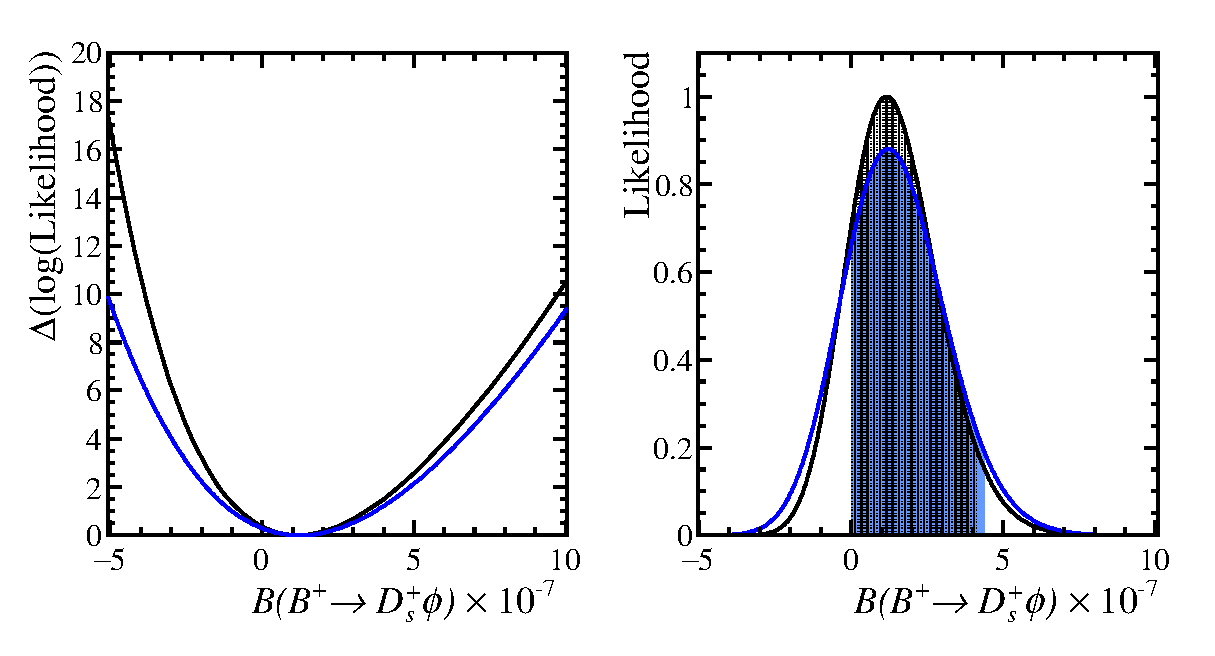
\includegraphics[width=1.0\textwidth]{figs/B2DsPhi/Likelihood_limits.eps}
        \caption{Bayesian profile likelihood limit determination}
    \label{fig:limit_likelihood}   
\end{figure}
%%%%%%%%%%%%%%%%%%%%%%%%%%%%%%%%%%%%%%%%%%%%%%%%%%%%%%%%%%

%%%%%%%%%%%%%%%%%%%%%%%%%%%%%%%%%%%%%%%%%%%%%%%%%%%%%%%%%%
\begin{figure}[!h]
    \centering
        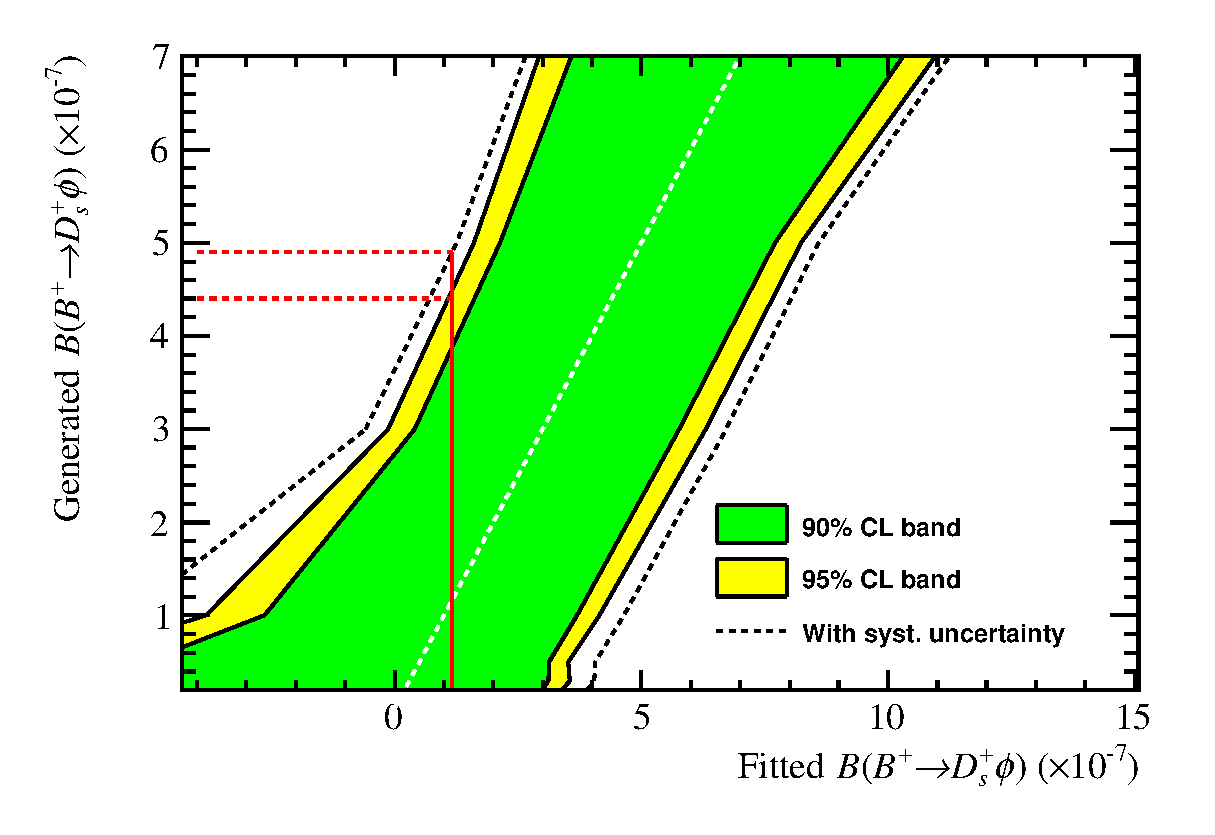
\includegraphics[width=0.8\textwidth]{figs/B2DsPhi/Sensitivity_plot.eps}
        \caption{CLs limit determination}
    \label{fig:limit_cls}   
\end{figure}
%%%%%%%%%%%%%%%%%%%%%%%%%%%%%%%%%%%%%%%%%%%%%%%%%%%%%%%%%%

\subsection{Comparison to 2011?}
